\documentclass[11pt]{article}
\usepackage[margin=1in]{geometry}
\usepackage{graphicx}
\usepackage{amsmath}
\usepackage[font=small,labelfont=bf]{caption}
\usepackage[colorlinks=true,allcolors=blue]{hyperref}
\usepackage{authblk}
\usepackage[round,authoryear]{natbib}
\usepackage{microtype}
\graphicspath{{polyrhythm_figs/}}
\renewcommand{\abstractname}{\vspace{-1.5em}}

\title{\bfseries Sound measurement of polyrhythmic phase coupling in biosignals:\\
diagnosing and correcting an \textit{n:m} coupling estimator}
\author[ ]{Antoine Bellemare-Pepin \and collaborators}
\affil[ ]{\small \textit{Draft for internal review --- numbers are quick-grade pending a paper-grade rerun.}}
\date{}

\begin{document}
\maketitle

\begin{abstract}
\noindent
Many biological rhythms do not merely co-occur but lock into integer \textit{n:m} polyrhythms: the heart
beats a fixed number of times per breath, cortical activity phase-locks to tremor, and stride entrains to
ventilation. The coupling \emph{order} and its stability are clinically meaningful state variables ---
they grade anaesthetic depth, index autonomic and sleep regulation, track fetal maturation, and scale
with tremor severity. Yet the estimators in routine use are applied almost universally without
validation against ground truth, and they are vulnerable to a fundamental confound: a single
non-sinusoidal oscillation decomposes into harmonics that are intrinsically phase-locked, so apparent
\textit{n:m} coupling can arise with no second oscillator at all. We treat \textit{n:m} coupling
\emph{measurement} as an object of study. We first confirm, on real cardiorespiratory recordings, that
genuine polyrhythms are present and recoverable. We then show that the \emph{default} settings of a
representative estimator do not merely lose power but \textbf{anti-detect} a clean 2:3 lock, and we
trace and correct four independent defects. With the corrected estimator no single technique is best:
the \textit{n:m} phase-locking value (PLV) is the most sensitive detector on clean, unimodal locks and at
low signal-to-noise, but is \emph{blind by construction} to multimodal locks, where entropy- and
mutual-information indices recover the coupling it misses. Finally we quantify the harmonics confound:
within one non-sinusoidal signal every technique false-positives, and no standard surrogate fully
removes it --- so \textit{n:m} coupling is soundly interpretable only between independent sources. We
release a validated cross-signal detector (a technique panel with surrogate inference and a scope guard)
and concrete recommendations.
\end{abstract}

\section{Introduction}

When two oscillations of different frequency interact, they need not lock only at 1:1. They can settle
into a rational \textit{n:m} regime --- $n$ cycles of one rhythm to $m$ of the other --- a polyrhythmic
form of synchronization. This was first made measurable in physiology by the cardiorespiratory
synchrogram, which revealed long, hidden epochs of 2:1 through 5:1 heartbeat-to-breath locking in
resting humans \citep{schafer1998,schafer1999}. The same \textit{n:m} formalism, equipped with a
noise-tolerant detector \citep{tass1998}, exposed pathological cortico-muscular locking in Parkinsonian
tremor; \textit{n:m} coupling has since been documented between maternal and fetal heartbeats
\citep{vanleeuwen2009}, between stride and breath in running \citep{bramble1983}, and, more
contentiously, across frequency bands in the brain \citep{palva2005,belluscio2012}.

The coupling order and its stability are not incidental. The cardiorespiratory ratio shifts in an
orderly cascade ($2{:}1\to3{:}1\to4{:}1\to5{:}1$) with anaesthetic depth; cardiorespiratory phase
synchronization indexes vagal/autonomic regulation and is altered in heart failure and diabetic
autonomic neuropathy; it is sleep-stage dependent and disrupted in sleep apnoea; maternal--fetal
coupling tracks fetal autonomic maturation; and cortico-muscular \textit{n:m} synchronization scales
with tremor severity and is a target for deep-brain stimulation \citep{schnitzler2005,purdon2013}.
Measuring \textit{n:m} coupling reliably is therefore of direct clinical and scientific value.

Two problems recur. First, the estimators --- the \textit{n:m} phase-locking value, the Shannon entropy
of the phase-difference distribution, conditional-probability indices, and phase mutual information ---
are assembled from a phase estimator, a ratio rule and a coupling statistic, each with defaults, and
applied to data without checking that they recover a \emph{known} polyrhythm. Second, a single
non-sinusoidal rhythm contains harmonics that are phase-locked by construction, so any \textit{n:m}
statistic computed within one signal can report ``coupling'' that is merely waveform shape ---
the confound emphasized by \citet{aru2015}, \citet{schefferteixeira2016} and \citet{cole2017}, and
compounded by surrogate nulls whose construction is neither standardized nor robust.

Here we make the measurement itself the experiment. Using cardiorespiratory recordings and polyrhythmic
ground truth with controllable ratio, coupling strength, waveform and noise, we ask, of a representative
estimator and of the broader technique family: are polyrhythms present and recoverable in real
biosignals; does the estimator retrieve a known lock; which technique wins in which regime; and does it
survive the harmonics confound? The answers are, in order: yes; not with its defaults; it depends on the
regime; and only between independent sources. We turn each into a fix and ship a validated detector.

\section{Results}

\subsection{Polyrhythms are present in real biosignals}

We first verify that the target phenomenon exists and is recoverable. On the PhysioNet \textit{Fantasia}
young-adult recordings we extracted the cardiac phase (linear between successive R-peaks) and the
respiratory phase (Hilbert analytic phase of cleaned respiration), and tested, per subject, the single
\textit{n:m} ratio predicted by that subject's heart/breath frequency ratio (avoiding
multiple-comparison inflation). A sliding-window synchronization index recovers genuine, intermittent
locking: the clearest subject shows a $1{:}3$ lock (three heartbeats per breath, matching the $3.2$
frequency ratio) with a windowed resultant reaching $R_{\max}=0.96$, significant against a cyclic-shift
surrogate null ($p=0.005$; Figure~\ref{fig:cardio}). Consistent with the classical finding that
cardiorespiratory synchronization is intermittent and subject-dependent
\citep{schafer1998,schafer1999}, not every resting subject locks at the predicted ratio. The phenomenon
is real; the rest of the paper asks whether our instruments measure it soundly.

\begin{figure}[t]
\centering
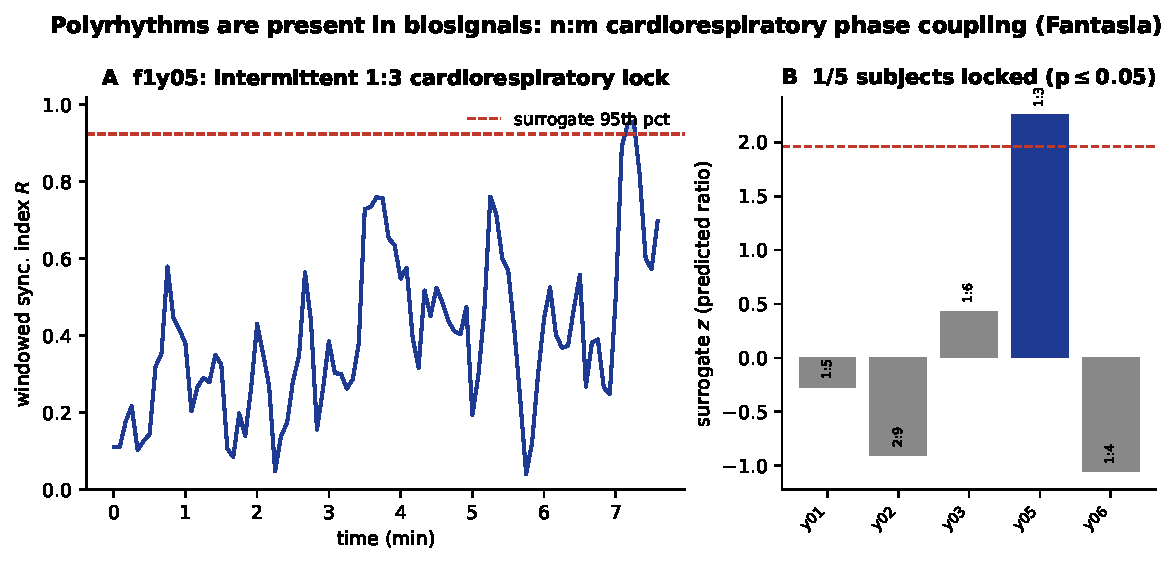
\includegraphics[width=\linewidth]{fig1_cardiorespiratory.pdf}
\caption{\textbf{A genuine \textit{n:m} polyrhythm in a real biosignal.}
(A) Sliding-window cardiorespiratory synchronization index for the clearest subject: epochs in which the
windowed resultant of the $1{:}3$ relative phase exceeds the surrogate 95th percentile mark genuine
intermittent locking. (B) Per-subject surrogate $z$ at the frequency-predicted ratio; cardiorespiratory
locking is intermittent and subject-dependent.}
\label{fig:cardio}
\end{figure}

\subsection{Default settings anti-detect a clean polyrhythm}

On synthetic ground truth --- a genuine 2:3 lock between two independent oscillators --- an oracle (the
\textit{n:m} PLV on band-pass--Hilbert phase at the known ratio) separates coupled from uncoupled cleanly
($\Delta=0.76$). The representative estimator's \emph{default} configuration does the opposite: coupled
signals score \emph{below} their uncoupled controls ($\Delta=-0.09$; Figure~\ref{fig:defaults}A). Four
independent defects explain it. (i)~\emph{Convention}: the ratio rule returns multipliers under a swapped
convention applied literally, so the relative phase is non-stationary even for a perfect lock; across the
ratio range every raw technique anti-detects ($\mathrm{AUC}\approx0.13$; Figure~\ref{fig:defaults}B).
(ii)~\emph{Phase estimator}: the default short-time-Fourier-transform bin phase is leakage-limited and
misses \textit{n:m} locking the Hilbert estimator recovers. (iii)~\emph{Ratio coverage}: the default
ratio table reaches only 3:3 and silently relabels unmatched pairs as 1:1. (iv)~\emph{Weighting}: a
complexity weight multiplied into the coupling value caps a perfect 2:3 lock at $\approx0.17$. We correct
each (canonical multipliers, Hilbert phase, exact-fraction ratios, unweighted readout).

\begin{figure}[t]
\centering
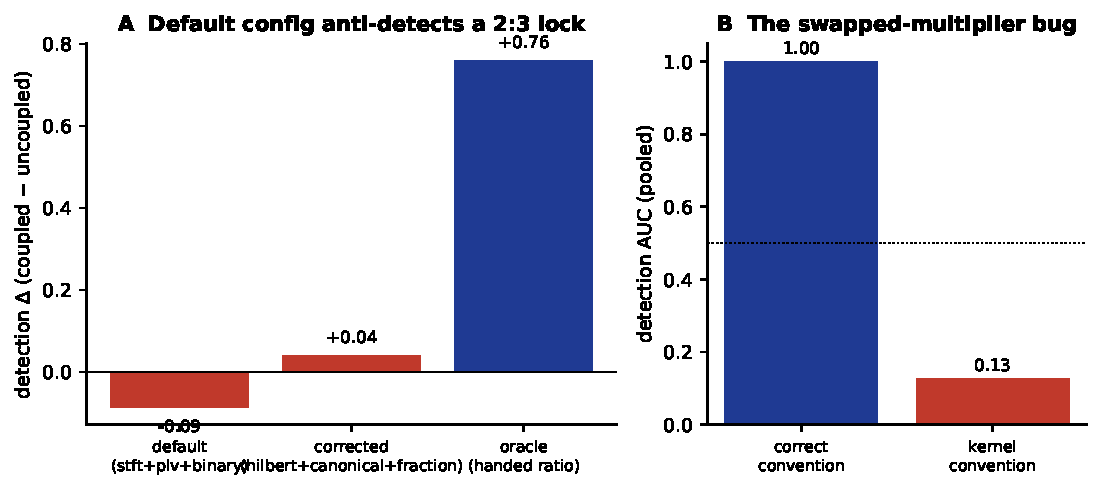
\includegraphics[width=0.92\linewidth]{fig2_defaults_fail.pdf}
\caption{\textbf{Default settings anti-detect a known lock.}
(A) Detection margin (coupled $-$ uncoupled) for a clean 2:3 lock: the default configuration is negative
(anti-detection), the corrected configuration recovers the sign, the oracle separates cleanly.
(B) The swapped-multiplier convention alone drives detection below chance; the canonical convention
restores it.}
\label{fig:defaults}
\end{figure}

\subsection{The corrected estimator is sound across the ratio range}

With the canonical convention, the \textit{n:m} PLV detects every tested lock from 1:2 through 5:7 at
ceiling, identifies the true ratio against a grid of candidate multipliers with near-perfect accuracy,
rises monotonically with coupling strength, and remains reliable to low SNR (Figure~\ref{fig:sound}).
The zero-lag-robust variants recover the lock at most ratios but plateau below ceiling; their robustness
to instantaneous mixing buys little here because, at $n\neq m$, the two channels are read at different
frequencies.

\begin{figure}[t]
\centering
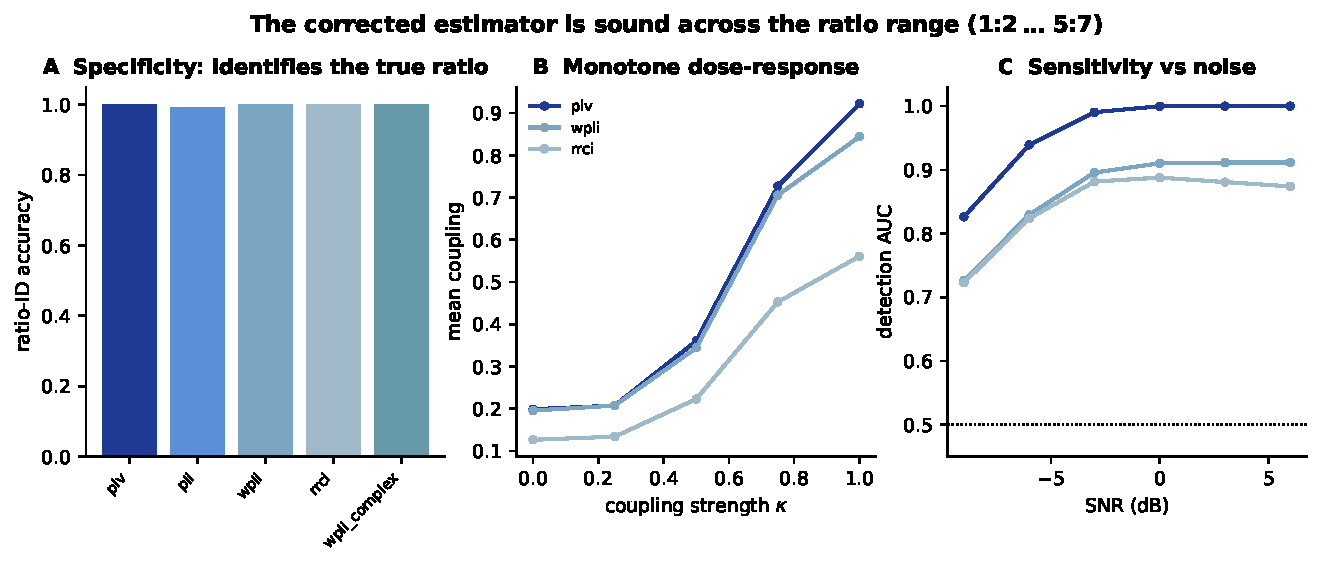
\includegraphics[width=\linewidth]{fig3_corrected_sound.pdf}
\caption{\textbf{The corrected estimator is sound.} (A) Ratio-identification accuracy across techniques.
(B) Monotone dose-response in coupling strength $\kappa$. (C) Detection AUC versus SNR; the PLV reaches
ceiling by $0$~dB.}
\label{fig:sound}
\end{figure}

\subsection{No single technique is best --- the winner is regime-dependent}

Across eight coupling regimes the techniques split into two families with complementary failure modes
(Figure~\ref{fig:regime}). On clean unimodal locks --- and under non-sinusoidal coupling, non-stationary
drift and added harmonics --- the PLV is supreme ($\mathrm{AUC}=1.00$) and is the most sensitive at low
SNR. But when the lock is \emph{multimodal} (a multistable or antipodal relative phase) the PLV and the
conditional-probability index \emph{anti-detect} ($\mathrm{AUC}\approx0.34$), because a balanced
multimodal distribution is \emph{less} unimodally concentrated than the independent null. Here the
all-moment indices dominate: the entropy index and phase mutual information recover the coupling
($\mathrm{AUC}\,0.90$--$0.99$) where every first-moment statistic fails. Weak graded coupling is genuinely
hard for all techniques. The practical reading is a \emph{panel}: the PLV for sensitivity on clean locks
and at low SNR, the entropy/information indices for generality against multimodal locks. This pattern was
reproduced independently, with separate generators and AUC code, under adversarial verification.

\begin{figure}[t]
\centering
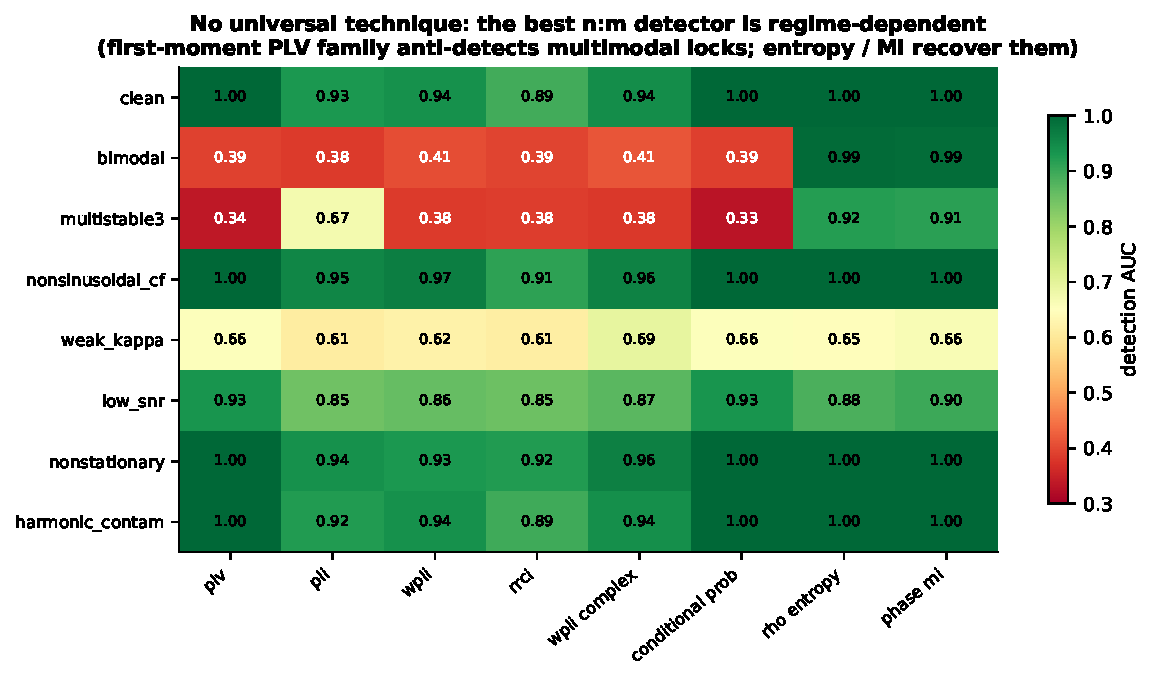
\includegraphics[width=0.86\linewidth]{fig4_regime_technique.pdf}
\caption{\textbf{No universal technique.} Detection AUC for eight techniques (columns) across eight
coupling regimes (rows). The first-moment PLV family (left) is supreme on unimodal-style regimes but
anti-detects the multimodal ones (\textit{bimodal}, \textit{multistable3}), where the all-moment entropy
and mutual-information indices (right) dominate.}
\label{fig:regime}
\end{figure}

\subsection{Within one signal, every technique false-positives --- and no surrogate fully fixes it}

A single non-sinusoidal oscillator has harmonics that are phase-locked by construction. Tested for
``1:2 coupling'' between its fundamental and second harmonic, \emph{every} technique reports strong,
significant coupling against an IAAFT null (surrogate $z$ of $7$, $42$ and $37$ for the PLV, entropy and
mutual-information indices; all 100\% significant; Figure~\ref{fig:confound}A), although there is only one
rhythm. The IAAFT null is the wrong control: it randomizes the cross-frequency phase relation, so a
signal's genuine harmonic lock appears ``coupled'' relative to the surrogate. Testing which null
separates artifact from genuine coupling, no standard surrogate fully removes the artifact: a
waveform-preserving block-shuffle reduces it roughly eight-fold while keeping genuine coupling strongly
detectable, but a residual remains (Figure~\ref{fig:confound}B). Within-signal \textit{n:m} at
harmonically related frequencies is therefore fundamentally confounded with waveform shape. The sound
regime is cross-signal: between independent sources the IAAFT-of-one-channel null destroys a real
inter-signal relationship with no within-signal harmonic confound --- the regime in which the
ground-truth recovery above holds, and the regime our detector enforces.

\begin{figure}[t]
\centering
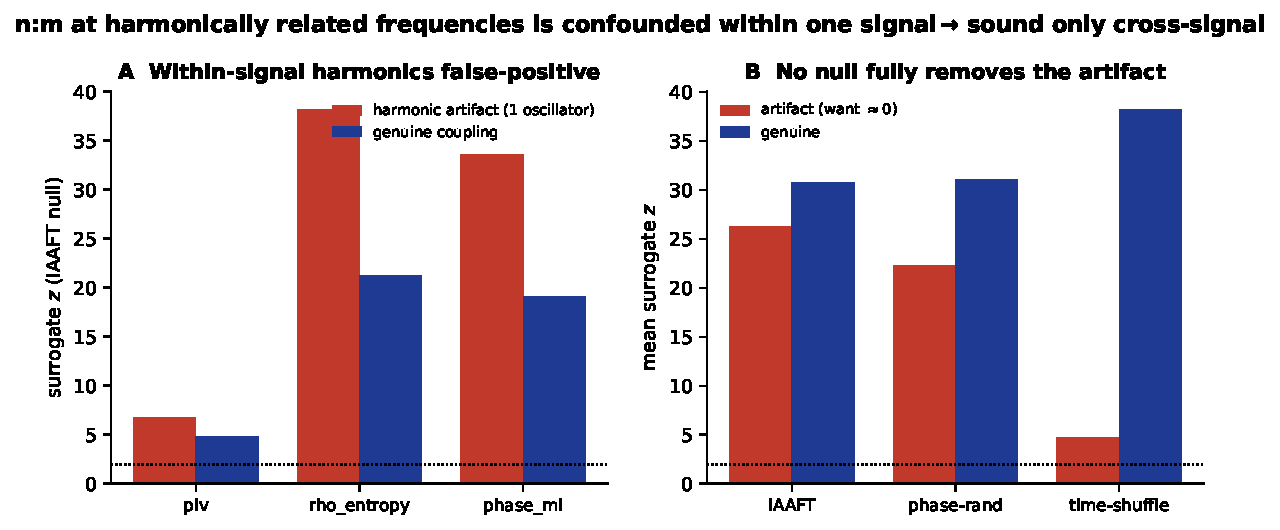
\includegraphics[width=\linewidth]{fig5_harmonic_confound.pdf}
\caption{\textbf{The harmonics confound.} (A) Within a single non-sinusoidal oscillator, every technique
reports significant ``\textit{n:m} coupling'' under an IAAFT null --- a false positive. (B) No standard
null removes it: IAAFT and phase-randomization fail badly; a waveform-preserving time-shuffle reduces the
artifact $\sim$8-fold but leaves a residual, while keeping genuine cross-signal coupling detectable.}
\label{fig:confound}
\end{figure}

\subsection{A validated detector}

We package these results as a cross-signal detector. It band-passes each component in its own band,
applies the canonical multipliers, reports a panel of complementary techniques (the PLV plus the entropy
and mutual-information indices), each with an IAAFT surrogate $z$ and rank-$p$, scans candidate ratios for
specificity, and emits an explicit scope-guard warning when the two inputs are too correlated to separate
coupling from shared-source harmonics. On held-out ground truth it recovers genuine locks across the
ratio range, stays null for independent signals and off-target ratios, detects the multimodal locks the
PLV alone misses, and warns on within-signal input. The detector and its regression tests are released in
the framework.

\section{Discussion}

Treated as an experiment, \textit{n:m} coupling \emph{measurement} yields three lessons. First, estimator
defaults can be not merely weak but \emph{directionally wrong}: a plausible pipeline anti-detected a
textbook polyrhythm, and the failure was invisible without ground truth. Second, there is \emph{no
universal \textit{n:m} statistic}: the first-moment PLV family and the all-moment entropy/information
family have complementary blind spots, so a panel --- not a single default --- is the honest instrument.
Third, the \emph{harmonics confound is a property of the design, not of the metric}: every technique
false-positives within one non-sinusoidal signal and no surrogate fully removes it, so the only sound
\textit{n:m} inference is between independent sources.

These results bear directly on the applications that motivate the measurement. A cardiorespiratory
synchrogram used to grade anaesthetic depth, an autonomic coupling index in heart failure, or a
cortico-muscular \textit{n:m} biomarker for deep-brain stimulation each rests on an estimator whose
defaults, technique choice and surrogate we show to be consequential; a directionally wrong default or a
harmonic false positive would corrupt the clinical readout. On the methodological critique that
cross-frequency coupling claims are confounded by waveform shape and inflated by mismatched surrogates,
the corrected estimator does not manufacture coupling where there is none, flags the within-signal regime
where it cannot be trusted, and reports surrogate-calibrated inference rather than a raw statistic.

\paragraph{Limitations.} The within-signal confound is scoped, not solved; a definitive within-signal test
would require waveform-aware controls beyond phase surrogates. Weak graded coupling sits near the
detection floor for all techniques. We did not implement a debiased estimator (pairwise phase consistency)
for comparing coupling across epochs of differing length, a useful addition where trial counts vary. The
real-data demonstration here is a single clearly-locked subject plus the established literature; a
population study across the full cohort and conditions (paced breathing, sleep, exercise) would
strengthen the prevalence estimate. All synthetic ground truth is at quick grade pending a paper-grade
rerun.

\begin{thebibliography}{99}
\small
\bibitem[Aru et al.(2015)]{aru2015} Aru J, Aru J, Priesemann V, Wibral M, Lana L, Pipa G, Singer W,
Vicente R (2015). Untangling cross-frequency coupling in neuroscience. \textit{Curr Opin Neurobiol}
31:51--61.
\bibitem[Belluscio et al.(2012)]{belluscio2012} Belluscio MA, Mizuseki K, Schmidt R, Diba K, Buzs\'aki G
(2012). Cross-frequency phase--phase coupling between theta and gamma oscillations in the hippocampus.
\textit{J Neurosci} 32:423--435.
\bibitem[Bramble \& Carrier(1983)]{bramble1983} Bramble DM, Carrier DR (1983). Running and breathing in
mammals. \textit{Science} 219:251--256.
\bibitem[Cole \& Voytek(2017)]{cole2017} Cole SR, Voytek B (2017). Brain oscillations and the importance
of waveform shape. \textit{Trends Cogn Sci} 21:137--149.
\bibitem[Palva et al.(2005)]{palva2005} Palva JM, Palva S, Kaila K (2005). Phase synchrony among neuronal
oscillations in the human cortex. \textit{J Neurosci} 25:3962--3972.
\bibitem[Purdon et al.(2013)]{purdon2013} Purdon PL et al. (2013). Electroencephalogram signatures of
loss and recovery of consciousness from propofol. \textit{PNAS} 110:E1142--E1151.
\bibitem[Sch\"afer et al.(1998)]{schafer1998} Sch\"afer C, Rosenblum MG, Kurths J, Abel HH (1998).
Heartbeat synchronised with ventilation. \textit{Nature} 392:239--240.
\bibitem[Sch\"afer et al.(1999)]{schafer1999} Sch\"afer C, Rosenblum MG, Abel HH, Kurths J (1999).
Synchronization in the human cardiorespiratory system. \textit{Phys Rev E} 60:857--870.
\bibitem[Scheffer-Teixeira \& Tort(2016)]{schefferteixeira2016} Scheffer-Teixeira R, Tort ABL (2016).
On cross-frequency phase--phase coupling between theta and gamma oscillations in the hippocampus.
\textit{eLife} 5:e20515.
\bibitem[Schnitzler \& Gross(2005)]{schnitzler2005} Schnitzler A, Gross J (2005). Normal and pathological
oscillatory communication in the brain. \textit{Nat Rev Neurosci} 6:285--296.
\bibitem[Tass et al.(1998)]{tass1998} Tass P, Rosenblum MG, Weule J, Kurths J, Pikovsky A, Volkmann J,
Schnitzler A, Freund HJ (1998). Detection of \textit{n:m} phase locking from noisy data: application to
magnetoencephalography. \textit{Phys Rev Lett} 81:3291--3294.
\bibitem[van Leeuwen et al.(2009)]{vanleeuwen2009} van Leeuwen P et al. (2009). Influence of paced
maternal breathing on fetal--maternal heart rate coordination. \textit{PNAS} 106:13661--13666.
\bibitem[Vinck et al.(2010)]{vinck2010} Vinck M, van Wingerden M, Womelsdorf T, Fries P, Pennartz CMA
(2010). The pairwise phase consistency: a bias-free measure of rhythmic neuronal synchronization.
\textit{NeuroImage} 51:112--122.
\end{thebibliography}

\end{document}
